\clearpage
\subsection{Euler angles and Quaternions}
\subsection*{Euler angles}
มุมออยเลอร์เป็นมุม 3 มุมที่คิดโดย Leonhard Euler เพื่อที่จะเอาไว้ใช้อธิบายการเอียงของวัตถุในปริภูมิ
ใช้ตัวแปรเพียงแค่ 3 ตัวเท่านั้น การบอกมุมออยเลอร์สามารถบอกได้หลายวิธี ในที่นี้เราใช้ ZYX Euler angles
ในการอธิบายมุมเอียงของเฟรมอ้างอิงที่เราสนใจเทียบกับเฟรมอ้างอิงเฟรมอื่น มุมออยเลอร์เกิดจากการหมุนเฟรมรอบแกนสามแกน
มาหมุนเรียงต่อกัน ต่อไปจะเป็นการรวมแมทริกการหมุนสามแกนเข้าด้วยกัน

\begin{equation}
	{R_{x}(\phi) = \begin{bmatrix}
		1 & 0 & 0 \\
		0 & c(\phi) & -s(\phi) \\
		0 & s(\phi) & c(\phi)
		\end{bmatrix}}
	\label{equ:rotation_matrix_x}
\end{equation}

\begin{equation}
	{R_{y}(\theta) = \begin{bmatrix}
		c(\theta) & 0 & s(\theta) \\
		0 & 1 & 0 \\
		-s(\theta) & 0 & c(\theta)
		\end{bmatrix}}
	\label{equ:rotation_matrix_y}
\end{equation}

\begin{equation}
	{R_{z}(\psi) = \begin{bmatrix}
		c(\psi) & -s(\psi) & 0 \\
		s(\psi) & c(\psi) & 0 \\
		0 & 0 & 1 \\
		\end{bmatrix}}
	\label{equ:rotation_matrix_z}
\end{equation}

โดยที่ $c(\phi) = cos(\phi)$, $s(\phi) = sin(\phi)$, $c(\theta) = cos(\theta)$, $s(\theta) = sin(\theta)$, $c(\psi) = cos(\psi)$, $s(\psi) = sin(\psi)$
จากแมทริกการหมุนแสดงให้เห็นว่า \quotes{Inertial frame} และ \quotes{ฺBody frame}
มีความสัมพันธ์กันเป็นแมทริกการหมุนคือ $R_{zyx}(\phi,\theta,\psi)$
\begin{equation}
	\begin{array}{c}
		{R_{zyx}(\phi,\theta,\psi) = R_{z}(\psi)R_{y}(\theta)R_{x}(\phi)}\\
		{= \begin{bmatrix}
		c(\theta)c(\psi) & s(\phi)s(\theta)c(\psi)-c(\phi)s(\psi) & c(\phi)s(\theta)c(\psi)+s(\phi)s(\psi) \\
		c(\theta)s(\psi) & s(\phi)s(\theta)c(\psi)+c(\phi)s(\psi) & c(\phi)s(\theta)c(\psi)-s(\phi)c(\psi) \\
		-s(\theta)       & s(\phi)c(\theta)                       & c(\phi)c(\theta)                       \\
		\end{bmatrix}}
		\label{equ:rotation_matrix_zyx}
	\end{array}
\end{equation}

แมทริกจากสมการที่ \ref{equ:rotation_matrix_zyx} เป็นแมทริกที่อธิบายถึงการหมุนจาก \quotes{ฺBody frame} ไปยัง \quotes{Inertial frame}
ดังรูปที่ \ref{fig:quadroter_eulerangles}
\begin{figure}[htbp]
	\centering
	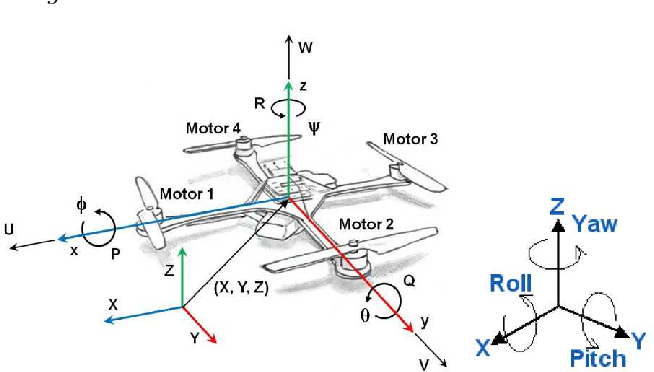
\includegraphics[width=0.65\textwidth]{images/Quadcopter_EulerAngles.png}
	\caption{ภาพแสดงการบอกแมทริกการหมุนของ Body frame}
	\label{fig:quadroter_eulerangles}
\end{figure}

\clearpage
\subsection*{Quaternions}
ในบางครั้งหรือบางกรณี Euler angles อาจจะทำให้เกิด Gimbal lock ได้
ซึ่งจะทำให้การควบคุมเสียไป 1 องศาอิสระ เพื่อที่จะหลีกเลี่ยงเหตุการณ์นี้จึงได้นำ quaternions มาใช้
quaternions ใช้เพื่อที่จะบอกมุมเอียงของวัตถุใดๆ ได้เหมือนกับ Euler angles
โดยที่เราสามารถแปลง Euler angles ให้เป็น quaternions ได้จากสมการที่ \ref{equ:euler2quat}

\begin{equation}
    {\begin{bmatrix} 
    q_1 \\ q_2 \\ q_3 \\ q_4
    \end{bmatrix} = \begin{bmatrix}
        c(\frac{\phi}{2})c(\frac{\theta}{2})c(\frac{\psi}{2})
        + s(\frac{\phi}{2})s(\frac{\theta}{2})s(\frac{\psi}{2}) \\[10pt]
        s(\frac{\phi}{2})c(\frac{\theta}{2})c(\frac{\psi}{2})
        + c(\frac{\phi}{2})s(\frac{\theta}{2})s(\frac{\psi}{2}) \\[10pt]
        c(\frac{\phi}{2})s(\frac{\theta}{2})c(\frac{\psi}{2})
        + s(\frac{\phi}{2})c(\frac{\theta}{2})s(\frac{\psi}{2}) \\[10pt]
        c(\frac{\phi}{2})c(\frac{\theta}{2})s(\frac{\psi}{2})
        + s(\frac{\phi}{2})s(\frac{\theta}{2})c(\frac{\psi}{2}) \\
		\end{bmatrix}}
	\label{equ:euler2quat}
\end{equation}

และเราสามารถที่จะเขียนแมทริกการหมุนให้อยู่ในรูปของ quaternions ได้ดังสมการที่ \ref{equ:quat2rot}
\begin{equation}
    {R_{zyx}(\phi,\theta,\psi) = \begin{bmatrix}
        q_1^2+q_2^2-q_3^2-q_4^2 & 2(q_2q_3-q_1q_4) & 2(q_1q_3+q_2q_4) \\[10pt]
        2(q_2q_3+q_1q_4) & q_1^2-q_2^2+q_3^2-q_4^2 & 2(q_3q_4-q_1q_2) \\[10pt]
        2(q_2q_4-q_1q_3) & 2(q_1q_2-q_3q_4) & q_1^2-q_2^2-q_3^2+q_4^2  \\
       \end{bmatrix}}
	\label{equ:quat2rot}
\end{equation}